\chapter{React – A JavaScript library for building user interfaces}
\label{cha:react}

This chapter introduces the reader to the prevalent and widespread front end library called ReactJS. It explains an essential part of React -- its rendering cycle -- which the reader needs to understand at least on a high level to be able to follow upcoming explanations of how the thesis project was implemented. Additionally, the paper elaborates the difference of how React uses declarative code to render data, whereas D3 uses an imperative API to render its data.

\section{Introduction to ReactJS}
\label{sec:reactIntro}

The easiest way to find information about React is to visit its official website \footnote{https://reactjs.org}. There is a statement in \cite{React} up front that says: \begin{quote}\begin{english}React is a JavaScript library for building user interfaces.\end{english}\end{quote} which describes React very well. A Facebook engineer called Jordan Walke founded the library in 2011, as presented in \cite[05:30]{ReactFoundingVideo}. Walke wanted to create a tool that would improve the code quality of their internal tool called ''Facebook ads''. Up until then, Facebook continued to develop and use React internally, but since the year 2013, the project is entirely open source. Since the initial open-source release up until now, not only technical engineers of Facebook but also the React open source community itself have been maintaining the library. In late 2017 Facebook even changed React's BSD license to the MIT license, which is even better for the React community, as the MIT license has lesser restrictions than the BSD license.

According to \cite{React}, Facebook sees React as a declarative and component-based library. However, a question might come to mind: ''What exactly does it mean for a library to be declarative and component-based?''. The answer to this question might be more straightforward than initially anticipated. In \cite{lloyd1994practical} declarative programming is described as a programming pattern, that expresses the logic of a program without describing its control flow. This means that the actual code only describes what has to be computed not necessarily how it should be done exactly by stating every action explicitly via a function call, for example. Declarative programming can be understood as a layer of abstraction, that makes software easier to understand for readers of the code. Declarative programming is therefore very different from the imperative programming pattern described in chapter \ref{cha:d3js}. React's approach of handling the presentation layer is declarative since its API lets developers describe how the application has to look like at any given data variation, which is quite the contrary to D3's API as it can be read in \ref{cha:d3js}. Further information about React's API can be found in section \ref{sec:reactApi} though.

Enabling developers to create a highly component oriented architecture in their software is a fundamental aspect of React as well. Using a component-based library can increase productivity a tremendous amount. However, what does it mean for a library to favor component based architecture? After the initial setup of some boilerplate code, React makes it exceptionally easy to reuse existing components in the codebase to allow even faster development cycles. Once standard input components like buttons or text fields and layout components like page or header components are implemented, they can be reused throughout the whole app; thus significant progress can be achieved in a very short amount of time. Components can be manipulated by passing different properties, which might result in different presentation results of the components. More in-depth information about how React handles components and its props can be found in section \ref{sec:reactApi}.

React components can have multiple applications. There are presentational components, for example, which are pure functions that represent the current application state. Though there are also stateful Components which can hold some application state and react to state changes accordingly via rendering again, react however makes no assumptions about the technology stack that is used in a project as \cite{React} claims. This means that users of the library can decide for themselves if they want to use the built-in state management functionality or if they want to use a third-party library for solving specific problems like global application state for example.

The documentation in \cite[/docs]{React} claims that the library makes use of a so-called ''virtual DOM''. This means that React keeps track of its state data to prevent unnecessary writes to the actual DOM object. JavaScript performs exceptionally well when handling pure JavaScript objects in memory. Keeping the DOM tree of the application in the JavaScript engine's heap as a representation of objects enables React primarily apply updates this so-called virtual DOM. React then compares the newly applied data with the old tree to then being able to decide updates need to be committed to the DOM. Writing or committing to the DOM is the most expensive type of work in the browser, so React tries to keep DOM manipulating actions to a minimum. The React team calls the diffing algorithm ''reconciliation algorithm''. It would go out of the scope of this paper to go more in depth of the algorithm, so it is recommended to read about React's reconciliation algorithm in its documentation \cite[/docs]{React}.

React is a view layer that favors unidirectional data-flow. Every time the application state changes, the whole new data object is passed to React again. As mentioned in \cite[6:50]{ReactFoundingVideo}, the speaker describes the functionality very well via explaining React as a simplified function that could look like this: \texttt{f(data) = UI}. Hence, React can be seen as the view layer that handles presentation as a function of state and data. Once the data has updated the virtual dom, the virtual dom is then passed to React's reconciliation algorithm, which then determines if any nodes have to be changed on the real DOM. If there would be a React component that always renders the same \texttt{<div>} with the same data, rendering that very component multiple times would not result in React writing multiple DOM nodes to the browser. The reconciliation algorithm sees that the virtual dom matches the real dom in this case, which results in React not updating the real DOM. Of course, if the component's content is dynamic, the component sometimes has to be re-rendered according to the data changes. If some parts of the data stay the same even after being reapplied to a component, only newly added or removed nodes are committed to the DOM. Even though the reconciliation algorithm prevents expensive DOM operations, the algorithm itself can also be expensive. The documentation in \cite[/docs/optimizing-performance.html\#avoid-reconciliation]{React} advises developers to try to avoid reconciliation to improve performance.

Unidirectional data-flow implicitly means to React developers, that there is no data binding and no template language. The library only uses \texttt{React.createElement([element])} calls internally, which are hidden behind the so-called ''JSX'' JavaScript language extension. JSX will be explained more i depth in section \ref{sec:reactApi}. As mentioned before, React is just a pure idempotent function of its application state, which means that the same data always produces the same presentation. That fact also implies that if the application data has to be changed, a new ''patched'' version of the application data has to be created instead of mutating the currently available application state. The newly created data then flows into the React render cycle again. Unidirectional data-flow is also the reason why React works well with immutable data structures. This paper assumes that the reader knows about immutable data structures, but \cite{ImmutableJS} explains exceptionally well, what Immutable data structures are and how they're used in JavaScript. Going more in-depth on how React works well with immutable state would go out of the scope of this thesis though. It is just essential to know that every time the data changes,  React triggers a whole new render cycle of the component tree. The immutable data structures help React to work out changes in the data structure when using immutable data structures. Instead of having to implement recursive data comparison functions, nested data object tree differences can be checked via a cheap equality check.

\section{Explaining the React API}
\label{sec:reactApi}

To follow performance discussions and elaborations about the thesis project's prototypes, a general high-level understanding of the API is required. This section introduces the reader to React's public API. The section does not aim to be a tutorial on how to program React applications, but rather to be a high-level explanation of how the API works. Reading this section makes it easy to understand the differences and similarities of React and D3 and how the two libraries play together and how they're also completely different.

\subsection{JSX in general}

\begin{program}
\caption{Creating a React element with JSX} 
\label{prog:reactJsxElement}
\begin{JsCode}
const ReactElement = (
  <div className="hello-world">
    Hello <span className="emph-text">World</span>!
  </div>
)
\end{JsCode}
\end{program}

\begin{program}
\caption{Creating a React element without JSX} 
\label{prog:reactJsxTranspiled}
\begin{JsCode}
const ReactElement = React.createElement(
  "div", 
  { className: "hello-world" }, 
  "Hello ", 
  React.createElement(
    "span", 
    { className: "emph-text" }, 
    "World"
  ), 
  "!"
);
\end{JsCode}
\end{program}

Probably one of the most important aspects of React's API is the JavaScript language extension called ''JSX'' which simplifies the use of React greatly and produces much more readable code. The example in \ref{prog:reactJsxElement} shows an example React component that is written in JSX. When looking at the transpiled output in \ref{prog:reactJsxTranspiled} it is clear how JSX helps to reduce the amount of code and how it greatly improves readability. The code in \ref{prog:reactJsxTranspiled} also shows that React is just a big composition of \texttt{React.createElement([element])} calls under the hood. When writing JSX code, in reality, it is writing declarative code that is just a functional composition of React components. 

Notice, how the createElement function takes up to 3 parameters as documented in \cite[/docs/react-api.html]{React}. The first parameter is the element type (the type can also be a custom component that was created by a user or a downloaded third-party component). The second parameter is used to pass the element's current properties, and the third parameter describes the component's children. That third parameter makes it possible to compose multiple React components together, as children are nestable. 

Line 2 and 3 in \ref{prog:reactJsxTranspiled} show, how a React element is created. A node of type \texttt{''div''} is created and the property \texttt{\{className: ''helo-world''\}} is passed. Each parameter after Line 3 is a child of the created \texttt{<div>} node. The React element has 3 children which is demonstrated by the code example where the element is written in JSX in \ref{prog:reactJsxElement}. First, there is the string ''Hello '', then there is a \texttt{<span>} which also has children, and finally there is the exclamation mark string at the end. When going back to the transpiled code example in \ref{prog:reactJsxTranspiled}, lines 4 to 10 exactly show what kind of children are passed to React's element creating function. Notice, that the class property has to be ''className'' in JSX instead of ''class'' because JSX is \emph{not} HTML, but extended JavaScript. Something also worth looking at is line 5 in \ref{prog:reactJsxTranspiled}. A nested \texttt{createElement()} call shows, how components can be composed together.

Because JSX is a language extension, a transpiler step is needed to produce production code. The common tool to use is called ''Babel''. There is a caption in \cite{Babel} that says: \begin{quote}\begin{english}Use next-generation JavaScript today.\end{english}\end{quote} The documentation in \cite[/docs/en]{Babel} explains, how modern JavaScript features can be used in any JavaScript project. The code which includes those modern features is normalized and transpiled by Babel to also work in older browsers. The tool accomplishes this by transforming the JavaScript code via its core implementation but also via some third-party plugins. A babel plugin has been created to transform JSX components into the syntax that can be seen in the code in \ref{prog:reactJsxTranspiled}. Just as a side note, although JSX became popular in conjunction with React, there are also other web technologies that make use of JSX like Vue.js \footnote{https://vuejs.org/} for example.

\subsection{Explaining React components}
\label{sec:reactComponents}

React's components can be split up in two categories: stateful and stateless components. The following paragraphs explain the difference between the two types of components and how they can be used in a React application.

\subsubsection{Functional stateless components}

\begin{program}
\caption{Simple example of a React component and its usage} 
\label{prog:reactHelloWorld}
\begin{JsCode}
import React from "react";
import ReactDOM from "react-dom";

const HelloComponent = props => {
  const name = props.name;
  return <div>Hello World to {name ? name : "you"}!</div>;
};

const PageComponent = props => {
  props.customFn("I get passed to the handler function!");
  return (
    <div>
      <h1>{props.title}</h1>
      <div>{props.content}</div>
      here are my children: [{props.children}]
    </div>
  );
};

const App = () => {
  return (
    <PageComponent
      customFn={console.log}
      title="I render the title prop"
      content="I render the content prop"
    >
      <HelloComponent />
      <HelloComponent name={"Max"} />
    </PageComponent>
  );
};

const rootElement = document.getElementById("root");
ReactDOM.render(<App />, rootElement);  
\end{JsCode}
\end{program}

As mentioned before, React is an extremely component oriented web technology. The example code in \ref{prog:reactHelloWorld} includes a purely presentational component called ''HelloComponent'' on line 4, a page layout component called ''PageComponent'' on line 9, and the base App component called ''App'' on line 20. React enables developers to create reusable and configurable components by providing the possibility to pass an arbitrary number of props to components. Generally speaking, props are used to not only control presentational details like color or layout variations but also to configure some initial state for example or to pass some application state data to a textbox component for example.

Without going too deep into the details of how a React application is rendered, lines 33 and 34 in \ref{prog:reactHelloWorld} show, how the app component is rendered into a specific entry point in the static \texttt{index.html} page. The app component on line 20 renders the page layout component, passes a few props which should demonstrate what types of props are possible and then renders the \texttt{HelloComponent} twice inside the layout component. One time the \texttt{HelloComponent} receives the prop \texttt{name} and one time the property is omitted. The output of the hello world example can be seen in figure \ref{fig:reactHelloWorld}. 

\begin{figure}
  \centering
  
\includegraphics[width=0.35\columnwidth]{react001}
  \caption{React hello world sample output}
  \label{fig:reactHelloWorld}
\end{figure}

The example in \ref{prog:reactHelloWorld} visualizes, how components can be reused throughout the application with different configurations and in different arrangements. The page layout component could be declared in an individual file to be reused in every page of the app. Via props React provides a reliable mechanism to control static state of the components that receive the props.

One of the most important aspects of React is that props -- once they're passed to a component -- are static and immutable inside the receiving component as React's documentation in \cite[/docs/components-and-props.html\#props-are-read-only]{React} demonstrates. Components that only render props and don't manage their own application state can be seen as pure functions which render the exact data they receive every render cycle. Props could thus be understood as parameters of a pure function, leading us back to the previously explained context of the function \texttt{f(data) = UI} in \ref{sec:reactIntro}. Another important aspect of React's prop mechanism is that props cannot be changed inside the receiving component. Props that are passed into a component are immutable and trying to mutate them results in React not noticing any changes in the data and therefore not activating a new render cycle.

\subsubsection{Stateful components}

\begin{program}
\caption{Simple example of a React component and its usage} 
\label{prog:reactStateful}
\begin{JsCode}
import React from "react";
import ReactDOM from "react-dom";

const Count = props => (
  <div>
    <div>I render the count</div>
    <div>The count is currently {props.count}</div>
  </div>
);

class StatefulComponent extends React.Component {
  constructor(props) {
    super(props);
    this.state = {
      count: 1
    };
  }

  counterHandler = () => {
    this.setState(state => ({ count: state.count + 1 }));
  };

  render() {
    return (
      <div>
        <h1>{this.props.title}</div>
        <Count count={this.state.count} />
        <button onClick={this.counterHandler}>+1</button>
      </div>
    );
  }
}

const App = () => <StatefulComponent title={"Counter Example"} />;

const rootElement = document.getElementById("root");
ReactDOM.render(<App />, rootElement);
\end{JsCode}
\end{program}

\begin{figure}
  \centering
  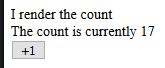
\includegraphics[width=0.25\columnwidth]{react002}
  \caption{React counter component output}
  \label{fig:reactCounterComponent}
\end{figure}

The attentive reader now probably has the following questions: ''How do I introduce mutable application state, if data coming from props is immutable?'' or ''How does React notice, if I introduce changes to the application state?''. At this point, it is important to remember, that React works best when keeping the unidirectional data-flow model in mind. The library provides a built-in mechanism for handling mutable application state out of the box. The code example in \ref{prog:reactLifecycleComponent} shows the difference between a purely presentational component on line 4 and a stateful component that keeps track of its application state on line 11.

First of, creating stateful components is quite effortless, as the component class simply derives from \texttt{React.Component} as shown in line 11 of the program in \ref{prog:reactStateful}. The constructor in line 12 calls its super constructor -- \texttt{React.Component} in that case -- and then initializes its state to \texttt{\{count: 1\}} right away even before the component has mounted for the first time. The state object is available throughout the whole class component and can be used to render UI components, that depend on that current state.

The example program in \ref{prog:reactStateful} demonstrates well, how the current state is used in the render method in line 23. Once the component calls its render method, the current state is accessed and rendered. Note, that the state cannot be altered and is immutable and read-only as well as the component's props. To introduce state changes, React provides a class member function which is called ''setState'', which takes a callback to update the internal component state as shown in line 20 of \ref{prog:reactStateful}. When the \texttt{this.setState} method is called, React is informed that there had been a state update and initiates a new render cycle which, as a consequence, triggers the whole lifecycle of the component again. The next section is all about React's lifecycle methods and how developers can utilize them.

% reconciliation?

% components do not have to have state for lifecycle components to work

\section{React's component lifecycle}

\begin{program}
\caption{Simple example of a React component and its usage} 
\label{prog:reactLifecycleComponent}
\begin{JsCode}
import React from "react";
import ReactDOM from "react-dom";

const Count = props => (
  <div>
    <div>I render the count</div>
    <div>The count is currently {props.count}</div>
  </div>
);

class StatefulComponent extends React.Component {
  constructor(props) {
    super(props);
    this.state = {
      count: 1
    };
  }

  componentDidMount() {
    console.log("I did mount.");
  }

  shouldComponentUpdate(nextProps, nextState) {
    return this.state.count !== nextState.count;
  }

  componentDidUpdate(prevProps) {
    console.log("I did uptate, previous props are", prevProps);
  }

  componentWillUnmount() {
    console.log("I am about to vanish...");
  }

  counterHandler = () => {
    this.setState(state => ({ count: state.count + 1 }));
  };

  render() {
    return (
      <div>
        <Count count={this.state.count} />
        <button onClick={this.counterHandler}>+1</button>
      </div>
    );
  }
}
  
const App = () => <StatefulComponent />;

const rootElement = document.getElementById("root");
ReactDOM.render(<App />, rootElement);  
\end{JsCode}
\end{program}

React components consist of a set of lifecycle methods that are called every render cycle of React, which is different from stateless functional components, as they are just pure functions. The previous code example in \ref{prog:reactStateful} was enhanced in \ref{prog:reactLifecycleComponent}. A few lifecycle methods -- some of which can be found on lines 19, 23, 27, 31, and 39 in \ref{prog:reactLifecycleComponent} -- make it possible to exactly control how components react to certain application state updates. Their names make it pretty clear what aspect of the lifecycle they handle.

React's documentation in \cite[/docs/react-component.html]{React} includes a comprehensive guide on component lifecycle methods. By overriding the lifecycle methods inside their components, developers can add their specific logic to each lifecycle in every render cycle of the components. Overriding lifecycle methods is optional; it is, therefore, possible to not implement any lifecycle method at all. Notice, how class components always have to override the \texttt{render()} function to being able to even render content. The render function is called every time the component goes through a new render cycle.

A good visualization of the full lifecycle of a React component can be found in the GitHub repo in \cite{ReactRenderCycleGithub}. The web application in \cite{ReactRenderCycleDiagram} visualizes the separation of the different phases a component goes through when iterating through its lifecycle methods. Figure \ref{fig:reactLifecycleMethods} shows a screenshot of the application for the sake of being able to demonstrate the diagram in the thesis. The diagram is based off a tweet in \cite{ReactCycleTweet} from Dan Abramov, one of the core contributors to the React library.

The whole lifecycle consists of 3 phases: The ''Render phase'', the ''Pre-commit phase'' and the ''Commit phase''. Also, the component can be in three different states: The mounting state, the updating state, and finally, the unmounting state. The visualization in \ref{fig:reactLifecycleMethods} shows the horizontal states and vertical phases of a React component. Every state of the component has to iterate all the phases each cycle vertically. Notice, how the update-render cycle does not call the constructor. What is also interesting is the fact, that the unmounting state only calls the \texttt{componentWillUnmount} method.

The most important lifecycle methods are \texttt{componentDidMount}, \texttt{componentDidUpdate} and \texttt{componentWillUnmount}. The \texttt{componentShouldUpdate} method is also important for improving performance, as explained later in this section. There are also more uncommon lifecycle methods for special occasions like the \texttt{getDerivedStateFromProps} method or the \texttt{getSnapshotBeforeUpdate} method. Those methods are rarely used and are not elaborated to avoid going out of the scope of this thesis. It is important to know, that the render phase is pure and can safely be aborted completely, resulting in a canceled lifecycle. Early cancelations of complete lifecycles can immensely improve performance.

The program in \ref{prog:reactLifecycleComponent} is a good demonstration of how lifecycle methods can be used. The lifecycle method on line 23, for example, controls, if the component should even go through it's rendering cycle or not. As mentioned before, Facebook advises avoiding reconciliation where ever possible. The \texttt{shouldComponentUpdate} lifecycle method already aborts the render cycle in the so-called ''render phase'' which allows developers to avoid unnecessary reconciliation cycles and therefore also commitments to the DOM. 

The \texttt{shouldComponentUpdate} method is the first lifecycle function that gets called in the example in \ref{prog:reactLifecycleComponent} aside from the constructor, which only gets called once in the mounting state of the component. The \texttt{shouldComponentUpdate} method gets passed all future props \emph{and} state which can then be compared to previous data. The example in \ref{prog:reactLifecycleComponent} shows, that the count from the current and the next state is compared and if they differ, \texttt{true} is returned, which means to React that a new render cycle is necessary. 

If for example the \texttt{StatefulComponent} on line 11 would have a parent that renders it 100 times, the stateful component is now smart enough to only run through its lifecycle methods only once, as \texttt{shouldComponentUpdate} method tells the component that nothing has changed and therefore omitting the rest of the lifecycle methods. Not calling the render function and its \texttt{createElement()} methods under the hood also has the implication, that no reconciliation has to be performed for the stateful component, resulting in improved rendering performance of the app.

The other lifecycle methods in the code example in \ref{fig:reactLifecycleMethods} are pretty self explanatory. There are a few best practices though, according to the documentation in \cite{React}. The \texttt{componentDidMount} method is the one to handle side effects when fetching data from an API, for example. Another use-case would be registering event handlers in the \texttt{componentDidUpdate} method and unregistering them in the \texttt{componentWillUnmount} method.

\begin{figure}
  \centering
  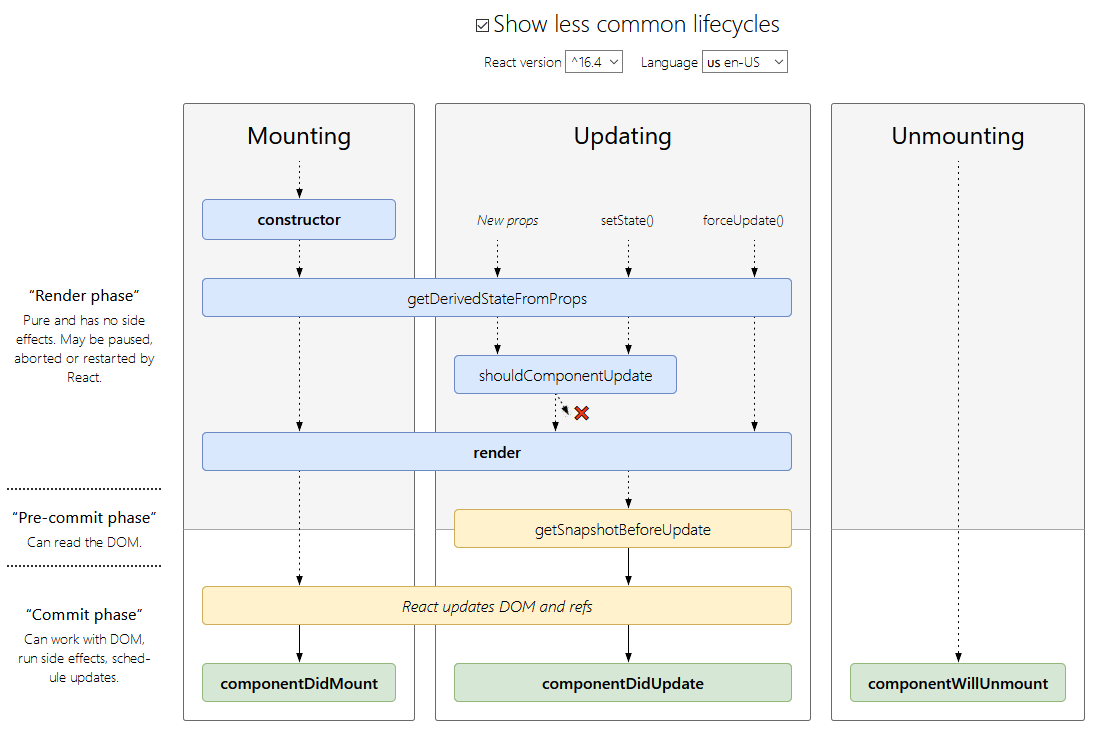
\includegraphics[width=1\columnwidth]{react003}
  \caption{React lifecycle methods diagram from \cite{ReactRenderCycleGithub}}
  \label{fig:reactLifecycleMethods}
\end{figure}

\section{Conclusion}

All in all, understanding the lifecycle of React components is a key aspect of also understanding how thesis project was implemented. Lifecycle methods play a crucial role when combining the rendering cycle of D3 with React's rendering cycle. It is essential to know that React has a virtual DOM, which it uses to compare virtual component trees to the real DOM to decide if any updates have to be committed to the DOM. Rendering a component with the same state multiple times results in React not committing anything to the DOM as the virtual DOM then equals the real DOM. It is also important to remember, that these so-called ''reconciliation cycles'' can completely be avoided by implementing the \texttt{shouldComponentUpdate} lifecycle method.

% what is state for the one component is immutable static prop for the other

%Another important aspect of React which is important for this project are its life cycle methods. Each component has a life cycle that will be executed on each rendering cycle. Developers can hook into those life cycle methods to implement some logic that should be executed after a component mounts or after a component was updated for example. The most well known life cycle methods of React are \texttt{componentDidMount()} or \texttt{componentDidUpdate()}.

% talk about animating stuff in react

% maybe introduce stateful functional components

% PureComponents? Hooks?

% \section{The difference between imperative and declarative APIs}
